\chapter{
(OLD) Introduction (to be converted over)
}\label{chp:Introduction}
%%%%%%%%%%%%%%%%%%%%%%%%%%%%%%
\section{Towards nature-based artificial intelligence}

\textit{Artificial intelligence} (AI) has progressed significantly in recent years due to massive increases in available computational power allowing the development and training of new deep learning algorithms \autocite{amodei2018ai}.
However, the best-performing learning algorithms often suffer from poor data efficiency and lack the levels of robustness and generalisation (\textit{i.e.,} poor transfer learning) that is characteristic of nature-based intelligence; reinforcement learning algorithms such as DeepMind’s AlphaZero algorithm \autocite{Silver2017a, Silver2017b} can successfully achieve superhuman level performance on many different games, however, they cannot transfer knowledge learnt during training on one game to another game: the system must be trained on each game individually\footnote{This algorithm shows generalisation during training, but no post-training generalisation (\textit{i.e.,} the same algorithm can learn to play different games with no code change, but knowledge learnt while training for one game cannot be transferred to a different but similar game).}.
Performance of current learning algorithms is also heavily dependent on intensive problem-specific feature engineering, which reduces the generalisation of their solutions to new problems and the speed at which novel applications can be constructed or tested.
Finally, current learning algorithms struggle, compared to nature-based intelligence, to learn tasks in dynamic, real-world environments by continually adapting their knowledge through interaction with their environment without experiencing catastrophic forgetting (\textit{i.e.,} they struggle with continual learning) \autocite{Sauders2018}; this is a long standing problem in reinforcement learning research and robotics.
A possible reason for the poor performance of these algorithms in replicating nature-based intelligence is that they are good at prediction using statistical, ‘model-free’ pattern recognition but not at building models, which can then be used to understand the world.
Processes that allow agents to build models of their environment, then continually update these models as time progresses, and the environment evolves, without explicit supervision appear the most promising path towards solutions to the described problems and towards human-like Artificial General Intelligence\footnote{Model-free approaches could be used to support model-building methods by accelerating inferences in perception and cognition, similar to how the occipital lobe processes data from the eye.} \autocite{Lake2017, Bengio2013}.

Improving the ability of an agent to generalise should allow for faster learning with improved data efficiency, which means that the artificial agent needs fewer data points to learn - especially important if the agent is learning in a real-world continual learning environment.
Improved generalisation can also increase the robustness of an agent's learning; this means that the agent reacts with greater consistency if it encounters data that is different, but similar, to the data that was used to train the agent.
This makes the agent's actions more predictable, since the agent should react in a similar way in real-world situations as it reacts in simulations or in controlled environments.
Therefore, it becomes easier to reduce the chance of the agent performing undesirable actions (\textit{e.g.}, an artificial agent running a self-driving car causing the car to drive off a bridge).
Robustness becomes increasingly important as artificial agents are used more and more for industrial applications.

%%%%%%%%%%%%%%%%%%%%%%%%%%%%%%
\section{Representation learning}

Much of the success of machine learning algorithms has been due to labour-intensive feature engineering of low-level sensory data, such as the creation of task-specific or data-specific data prepossessing pipelines which transform data into forms that are easier for current machine learning algorithms to learn.
This feature engineering relies on human-curated, task-specific prior knowledge because current learning algorithms struggle to identify and disentangle the underlying explanatory factors of the data.
If learning algorithms were less dependant on labour-intensive feature engineering, then novel applications could be constructed faster, and trained more efficiently.

\textit{Representation learning} (RL) is a process that transforms data into useful, (usually) more abstract features, which can faithfully characterise the data, into a form where it is easier to extract useful information for other algorithms, such as classifiers or predictors.
The transformed data is known as a \textit{representation} of the original data.
RL algorithms can be thought of as seeking to remove the need for human-curated, task-specific feature engineering by performing useful feature engineering automatically\footnote{This also means that, ideally, RL would be an unsupervised learning process.}.
RL is a wide domain that has had success in many applications across a range of areas, such as machine vision, speech recognition, natural language processing, and reinforcement learning (see \autocite{Bengio2013} for examples).

In state RL (a particular case of RL) features are low dimensional, evolve through time and are influenced by the actions of agents \autocite{Lesort2018StateRL}.
More formally, an agent uses sensors to form observations of the states of the environment (the observation process); these observations can then be used to create representations of the environment (the inference process) \autocite{Russell2010}.
Mathematically, this process can be described as a mapping from aspects of the world state (\textit{i.e.,} the environment) to the observations followed by a mapping from the observations to representations which can then be used by learning or control algorithms (see figure \ref{fig:intro-flow-chart}).
State RL has been combined with reinforcement learning to enable algorithms to learn more efficiently and with improved ability to transfer learnings to other tasks (improved generalisation) \autocite{Munk2016}.
It is hypothesised that the success of state RL is because the learned abstract representations are convenient to describe general priors about the world in a way that is easier to interpret and utilise while not being task specific; this makes the representations useful for solving a range of tasks \autocite{Bengio2013}.
It has also been argued that representations that express general priors about the world are necessary for progress towards Artificial General Intelligence.

\begin{figure}[H]
    \centering
    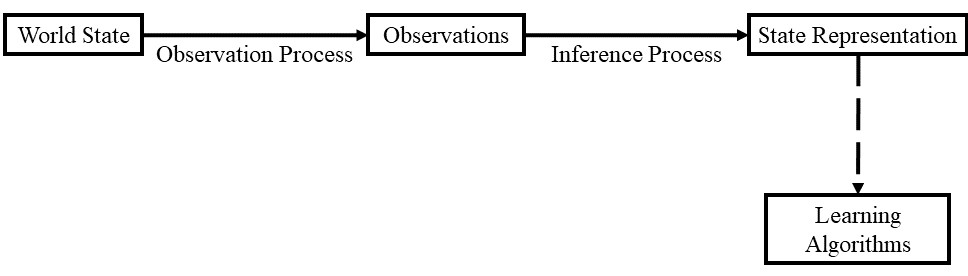
\includegraphics[width = \textwidth]{1Introduction/Old/Images/fig-intro-flow-chart.jpg}
    \caption{Diagram showing mappings from the world state to a state representation.}
    \label{fig:intro-flow-chart}
\end{figure}

%%%%%%%%%%%%%%%%%%%%%%%%%%%%%%
\section{Symmetries}

Due to their successes in Physics and other scientific disciplines, symmetries have been proposed as important aspects of the world that should be preserved in agents' representations, and as a method to disentangle representations \autocite{Higgins2018}.
The study of algebraic structures and symmetries and how these structures relate to the world around us has been extremely successful in the creation of accurate, interpretable representations of the universe in Physics; since symmetry transforms are prevalent at every level of abstraction they have been used to make predictions, test theories and discover previously unknown relationships between concepts.

This research is being conducted, in part, on the belief that there are properties of the transitions between world states that are true for any structure or, at least, that are true for large classes of structures, which share similar characteristics.
We believe that these universal properties have the potential to improve generalisation in the RL of a range of structures.

We believe that \autocite{Higgins2018}'s approach, of describing the structure of world states and their transitions in state representations using abstract mathematics (\textit{i.e.}, their use of groups and group representations), and \autocite{caselles2019symmetry}'s insights, of using \autocite{Higgins2018}'s approach to describe specific types of an agent's actions, can be recovered and extended by a more general mathematical framework built from first principles.
We believe that this mathematical framework will enable the description, and potentially the discovery, of universal properties of transitions between world states.
The discovery of such universal properties, aside from being interesting in their own right, could impact RL by informing improvements to RL algorithms (\textit{e.g.}, improving an agent's ability to generalise to new environments, or improving the performance of an agent in particular environments), by providing explanations for why certain algorithms can or cannot learn to the represent the details of particular structures, and by leading to the unification of different ideas in RL under a single framework.


%%%%%%%%%%%%%%%%%%%%%%%%%%%%%%%%%%%%%
\section{Mathematical background}\label{sec:Mathematical background}

%%%%%%%%%%%%%%%%%%%%%%%%%%%%%%
\subsection{Symmetries}

A symmetry is an intrinsic property of a mathematical object, where the object remains invariant to (unchanged by) certain transformations (\textit{e.g.}, rotations, reflections, more abstract transformations etc...) \autocite{Mathworld-group-theory}.

Mathematically, a symmetry is a mapping of an object to itself, which preserves the structure of the object.
If this object is a set, which has no additional structure, then a symmetry is a permutation of the elements in the set; this is equivalent to a bijective map from the set to itself.

%%%%%%%%%%%%%%%%%%%%%%%%%%%%%%
\subsection{Groups}

The concept of (full) symmetries can be described in abstract terms by the mathematical theory of groups.

\begin{definition}[Group]
    A group is a set $G$ together with a binary operation $\cdot$ that satisfies:
    \begin{itemize}
        \item \textbf{Closure/Totality:} $\forall g,h \in G, \ \ g \cdot h \in G$.
        \item \textbf{Associativity:} $\forall g,h,l \in G, \ \ (g \cdot h) \cdot l = g \cdot (h \cdot l)$.
        \item \textbf{Identity:} there exists an element $e \in G$ such that $e \cdot g = g \cdot e = g \ \ \forall g \in G$.
        \item \textbf{Inverse/Invertibility:} for each $g \in G$, there exists an element $g^{-1} \in G$ such that $g \cdot g^{-1} = g^{-1} \cdot g = e$.
    \end{itemize}
\end{definition}

Two groups $G$ and $H$ can be combined using the \textit{direct product} to give another group $G \times H$ with elements $(g, h)$ where $g \in G$ and $h \in H$.

To describe the effect of symmetry transforms on an object, a \textit{group action} is used.
The elements in the set $X$ in definition ref[def:group-action] would be aspects of the object (\textit{e.g.}, the corners of a shape) and the elements of $G$ are the transformations.

\begin{definition}[(left) Group action]\label{def:group-action}
     Let $(G, \cdot)$ be a group with identity element $1$, and let $X$ be a set.
     A (left) group action $\alpha$ of $G$ on $X$ is a function $\alpha: G \times X \to X$ that satisfies:
     \begin{enumerate}
         \item (Identity) $\alpha(1, x) = x$ for all $x \in X$;
         \item (Compatibility) $\alpha(g, \alpha(h,x)) = \alpha(g \cdot h, x)$ for all $g,h \in G$ and all $x \in X$.
     \end{enumerate}
\end{definition}

An important type of group action is a \textit{group representation}.
This is when a group acts on a vector space through invertible linear maps \autocite{Mathworld-group}.
The idea of group representations is notable because it can allow the representation of group transforms as the set of $n\times x$ invertible matrices along with the operation of matrix multiplication; matrices are commonly used in current ML algorithms.


%%%%%%%%%%%%%%%%%%%%%%%%%%%%%%
\subsection{Relaxing the properties of groups}\label{sec:Relaxing the properties of groups}

It might be desirable to use algebraic structures that do not require one or more of the properties of groups.
These more flexible algebraic structures can be used to describe processes that do not adhere to group properties.
See ref[fig:properties-of-groups-table] for a description of these more flexible group-like structures.

\begin{table}[H]
\begin{tabularx}{\textwidth}{|X|c|c|c|c|c|}
\hline
\rowcolor[HTML]{CFE2F3} 
\textbf{Group-like structures} & \textbf{Totality} & \textbf{Associativity} & \textbf{Identity} & \textbf{Invertibility} & \textbf{Commutativity} \\ \hline
Semigroupoid                  & \cellcolor[HTML]{F4CCCC}N  & \cellcolor[HTML]{D9EAD3}Y & \cellcolor[HTML]{F4CCCC}N  & \cellcolor[HTML]{F4CCCC}N  & \cellcolor[HTML]{F4CCCC}N  \\ \hline
Small Category                & \cellcolor[HTML]{F4CCCC}N  & \cellcolor[HTML]{D9EAD3}Y & \cellcolor[HTML]{D9EAD3}Y & \cellcolor[HTML]{F4CCCC}N  & \cellcolor[HTML]{F4CCCC}N  \\ \hline
Groupoid                      & \cellcolor[HTML]{F4CCCC}N  & \cellcolor[HTML]{D9EAD3}Y & \cellcolor[HTML]{D9EAD3}Y & \cellcolor[HTML]{D9EAD3}Y & \cellcolor[HTML]{F4CCCC}N  \\ \hline
Magma                         & \cellcolor[HTML]{D9EAD3}Y  & \cellcolor[HTML]{F4CCCC}N  & \cellcolor[HTML]{F4CCCC}N  & \cellcolor[HTML]{F4CCCC}N  & \cellcolor[HTML]{F4CCCC}N  \\ \hline
Quasigroup                    & \cellcolor[HTML]{D9EAD3}Y  & \cellcolor[HTML]{F4CCCC}N  & \cellcolor[HTML]{F4CCCC}N  & \cellcolor[HTML]{D9EAD3}Y  & \cellcolor[HTML]{F4CCCC}N  \\ \hline
Unital Magma                  & \cellcolor[HTML]{D9EAD3}Y  & \cellcolor[HTML]{F4CCCC}N  & \cellcolor[HTML]{D9EAD3}Y  & \cellcolor[HTML]{F4CCCC}N  & \cellcolor[HTML]{F4CCCC}N  \\ \hline
Loop                          & \cellcolor[HTML]{D9EAD3}Y  & \cellcolor[HTML]{F4CCCC}N  & \cellcolor[HTML]{D9EAD3}Y  & \cellcolor[HTML]{D9EAD3}Y  & \cellcolor[HTML]{F4CCCC}N  \\ \hline
Semigroup                     & \cellcolor[HTML]{D9EAD3}Y  & \cellcolor[HTML]{D9EAD3}Y  & \cellcolor[HTML]{F4CCCC}N  & \cellcolor[HTML]{F4CCCC}N  & \cellcolor[HTML]{F4CCCC}N  \\ \hline
Inverse Semigroup             & \cellcolor[HTML]{D9EAD3}Y  & \cellcolor[HTML]{D9EAD3}Y  & \cellcolor[HTML]{F4CCCC}N  & \cellcolor[HTML]{D9EAD3}Y  & \cellcolor[HTML]{F4CCCC}N  \\ \hline
Monoid                        & \cellcolor[HTML]{D9EAD3}Y  & \cellcolor[HTML]{D9EAD3}Y  & \cellcolor[HTML]{D9EAD3}Y  & \cellcolor[HTML]{F4CCCC}N  & \cellcolor[HTML]{F4CCCC}N  \\ \hline
Commutative Monoid            & \cellcolor[HTML]{D9EAD3}Y  & \cellcolor[HTML]{D9EAD3}Y  & \cellcolor[HTML]{D9EAD3}Y  & \cellcolor[HTML]{F4CCCC}N  & \cellcolor[HTML]{D9EAD3}Y  \\ \hline
Group                         & \cellcolor[HTML]{D9EAD3}Y  & \cellcolor[HTML]{D9EAD3}Y  & \cellcolor[HTML]{D9EAD3}Y  & \cellcolor[HTML]{D9EAD3}Y  & \cellcolor[HTML]{F4CCCC}N  \\ \hline
Abelian Group                 & \cellcolor[HTML]{D9EAD3}Y  & \cellcolor[HTML]{D9EAD3}Y  & \cellcolor[HTML]{D9EAD3}Y  & \cellcolor[HTML]{D9EAD3}Y  & \cellcolor[HTML]{D9EAD3}Y  \\ \hline
\end{tabularx}
\caption{Properties of various group-like algebraic structures (figure from \autocite{group_like_table}.).}
\label{fig:properties-of-groups-table}
\end{table}


Commutativivity is the property where for a group-like algebraic structure $(G, \circ)$ and for any $g,h \in G$ then $g \circ h = h \circ g$.

%%%%%%%%%%%%%%%%%%%%%%%%%%%%%%
\subsection{Category theory}

A category $C$ is a class of objects $ob(C)$ together with a class of morphisms that relate the objects to each other.
Two objects are associated with every morphism: the source, where the morphism starts, and the target, where the morphism ends.
Morphisms can be combined using a partial binary operation (`composition'); the composition $f \circ g$ of two morphisms $f, g$ is defined when the target of $g$ is the source of $f$.
Morphisms obey associativity: $h \circ (g \circ f) = (h \circ g) \circ f$.
The properties of morphisms are shown in fig \ref{fig:morphisms}.

\begin{figure}[H]
    \centering
    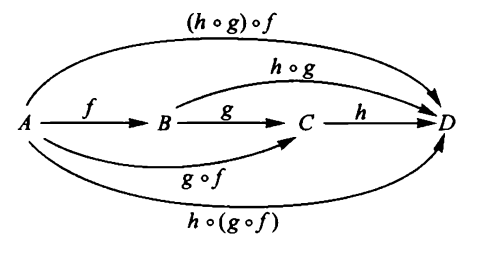
\includegraphics[scale = 0.8]{1Introduction/Old/Images/fig-morphisms.png}
    \caption{The morphism properties of composition and associativity \autocite{associativity2019}.
    $f$, $g$, and $h$ are morphisms of a category.
    $A$, $B$, $C$ and $D$ are objects of the category.}
    \label{fig:morphisms}
\end{figure}

A functor $F: C \to D$ between two categories $C$ and $D$ is a mapping that preserves identity morphisms and composition of morphisms \autocite{functor2020}:
\begin{itemize}
    \item Associates each object $X \in ob(C)$ to an object $F(X) \in D$.
    \item Associates each morphism $f: X \to Y$ in $C$ to a morphism $F(f): F(X) \to F(Y)$ in $D$ such that $F$ satisfies:
    \begin{itemize}
        \item $F(id_{X}) = id_{F(X)}$ for every object $X \in ob(C)$.
        \item $F(g \circ f) = F(g) \circ F(f)$ for all morphisms $f: X \to Y$ and $g: Y \to Z$ in $C$.
    \end{itemize}
\end{itemize}

A natural transform $\eta$ between two functors $F: C \to D$ and $G: C \to D$ consists of the morphisms $\eta_{x}: F(x) \to G(x)$ for each object $x \in C$ that obey the property $G(f) \circ \eta_x = \eta_y \circ F(f)$ for each morphism $f: x \to y$ in $C$ \autocite{natural_transform2020}.

A homomorphism is a map $f: A \to B$ between sets $A, B$ that preserves the operation $\cdot$ by satisfying: $f(x, y) = f(x) \cdot f(y)$ for every pair $x, y \in A$.

An isomorphism is a bijective homomorphism (\textit{i.e.,} a morphism that has an inverse that is also a morphism).


%%%%%%%%%%%%%%%%%%%%%%%%%%%%%%
\section{What makes a good representation?}\label{sec:What makes a good representation?}

%%%%%%%%%%%%%%%%%%%%%%%%%%%%%%
\subsection{Priors for representations}

\autocite{Bengio2013} proposed that representations that express general priors about the world could be useful for a large range of AI and robotics tasks.
Examples of possible general priors, or properties, proposed include:
        % #TODO: define mathematical formalism for these conditions (what is $f$ ?, what is $x$ ? etc...)
\begin{enumerate}
    \item \textbf{Smoothness.}
    The assumption that the function $f$ being learned satisfies the property: $x \approx y \implies f(x) \approx f(y)$, where $x,y$ are input data points.
    Smoothness exploits the principle of local generalisation, which is the assumption that the target function is smooth enough so that training examples can be used to explicitly map out the variations of the target function.
    
    \item \textbf{Multiple explanatory factors.}
    The data generating the distribution is generated by many different underlying factors.
    In many cases, what is learnt about one of the underlying factors can generalise to the other factors.
    
    \item \textbf{Hierarchical organisation of explanatory factors.}
    Concepts used to describe the world can be defined in terms of other concepts.
    Concepts that are higher in the hierarchy are considered to be more abstract because they are constructed from concepts at lower levels of the hierarchy rather than being built using the raw input data.
    
    \item \textbf{Semi-supervised learning.}
    For a supervised learning problem with input data $X$ and targets $Y$ to predict, a subset of the underlying factors that explain the distribution of $X$ explain how the targets $Y$ can be obtained from $X$ (\textit{i.e.}, some underlying features of the input data $X$ can be used to identify the target for a specific piece of data).
    Therefore, representations that describe the distribution $P(X)$ of $X$ tend to be useful when learning $P(Y \mid X)$.
    This can be viewed as the unsupervised learning task of producing a representation of $X$ sharing statistical strength with the supervised learning task of predicting the targets $Y$ given the data $X$.
    
    \item \textbf{Manifolds.}
    The probability mass concentrates near regions that form a much lower dimensional space than the original data space.
    These lower dimensional spaces can be interpreted as manifolds\footnote{In other words, the behaviour space of the model has a much lower dimensionality than the input space to the model.}.
    This is a key assumption of the manifold learning paradigm of RL (see section \ref{sec:manifold-learning}).
    
    \item \textbf{Temporal and spatial coherence.}
    Consecutive observations or spatially close observations result in a small movement on the surface of the high-density representation manifold.

    Also, it has been proposed that different underlying explanatory factors of the data distribution could change at different time scales and different spatial scales; this could possibly be exploited to disentangle explanatory factors (see section \ref{sec:Disentangled representations}).
    
    It is also expected that some explanatory factors of the data would be represented by a collection of values (\textit{e.g.}, the $x$, $y$, and $z$ positions of an object in space) which would spatially and temporally move together.
    Additionally, it is sometimes assumed that many concepts of interest change (relatively) slowly; these concepts can be captured in a representation by making the constructed representation change slowly through penalising changes in values over space and time.

    \item \textbf{Sparsity.}
    For any given observation $x \in X$, only a small fraction of possible factors are relevant and this should be reflected in representations of the data distribution that produced the observations.
    
    This sparsity property could appear in representations by underlying features, or combinations of underlying features, that are often zero for a given observation, or by the value of most of the extracted underlying features in the representations not changing significantly due to small variations in observations.
    
    A potential method for enforcing this sparsity property on representations is by penalising the magnitude of the Jacobian matrix (of derivatives) of the function mapping input to representation.
    
    \item \textbf{Simplicity of factor dependencies.}
    In high-level representations, it is sometimes considered good if the underlying factors are related to each other through simple, typically linear, dependencies.
    This also has the benefit of making the construction of algorithms easier since computers are very good at linear algebra manipulation (\textit{e.g.}, matrix multiplication).
    
    \item \textbf{Expressiveness.} Good representations can accurately capture a large number of input configurations. This can be measured by counting the number of parameters the model requires compared to the number of input regions it can distinguish \autocite{luo2019expressiveness}.
\end{enumerate}


% \begin{itemize}
%     \item Temporal coherence prior
%     \begin{itemize}
%         \item ``The principle of identifying slowly moving/changing factors in temporal/spatial data has been investigated by many as a principle for finding useful representations.''
        
%         \item Simplest expression of temporal coherence prior: penalise the squared difference between underlying feature values at times $t$ and $t+1$.
        
%         \item Can also penalise separate underlying factors by different time scales, and the difference in these time scales could help in disentangling the explanatory factors.
        
%         \item Would also expect that some factors would be represented by collections of numbers rather than a single scalar.
%         These collections of number would be expected to tend to move together  (see ``structured sparsity penalities'').
%     \end{itemize}


    
%     \item Disentangling features
%     \begin{itemize}
%         \item Low-level features recovered. Then subsets of low level-features used to give higher-level features with greater invariance.
%     \end{itemize}
% \end{itemize}

%%%%%%%%%%%%%%%%%%%%%%%%%%%%%%
\subsection{Disentangled representations}\label{sec:Disentangled representations}

Many of these potential priors can be viewed as ways for the learner to separate out some of the underlying factors of variation in the data so that certain changes in the input data only change some aspects of the representation of that input data point, but do not change other aspects; representations with this property are called \textit{disentangled representations}.
\textit{Disentangled RL} aims to produce representations that disentangle as many factors of some original data as possible, while discarding as little information as possible from the original data \autocite{Bengio2013}.

%%%%%%%%%%%%%%%%%%%%%%%%%%%%%%
\subsection{Generalisation}

As stated previously, the smoothness property allows learning algorithms to use the principle of local generalisation by using training data to map out the variations in the, assumed to be, smooth target function.
Local generalisation relies on local interpolation between neighbouring training examples to make predictions for unseen data.
However, this smoothness assumption falls down when it encounters data with many interacting underlying features, which are relevant to the prediction of the target function, because the number of changes in the target function commonly grows exponentially with the number of relevant interacting underlying features when the data are represented in the raw input space; this is a case of the \textit{curse of dimensionality}.

%%%%%%%%%%%%%%%%%%%%%%%%%%%%%%
\subsection{Abstraction through deep architectures}

\textit{Deep architectures} have a natural hierarchy, which can lead to abstract representations as more abstract concepts are constructed in terms of less abstract concepts.
More abstract concepts are generally invariant to local changes of the initial input data compared to less abstract concepts.
This generally makes representation that capture more abstract concepts highly non-linear functions of the raw input.

Deep architectures also promote the re-use of features, which encourages the construction of more abstract representation at deeper levels of the architecture.
Also, since the number of ways to use features at different depths of a deep architecture grows exponentially as the depth of the architecture grows (\textit{i.e.}, the number of ways to use different parts of the architecture grows exponentially with the depth of the architecture), using deep architectures can give improvements in computational efficiency (fewer nodes to visit for the model give its output) and statistical efficiency (fewer model parameters to learn), which both improve computational performance.

%%%%%%%%%%%%%%%%%%%%%%%%%%%%%
\section{Paradigms for RL}\label{sec:Paradigms for RL}

In this section we provide an overview of some approaches to RL:
\begin{enumerate}
    \item \textbf{Probabilistic models.}
    This approach to RL seeks to directly parametrise the decoding map (\textit{i.e.}, the generative map).        % #TODO: change name to more general version ?
    
    \item \textbf{Parametrising a representation function.}
    This approach to RL uses seeks to directly parametrise the encoding map.
    
    \item \textbf{Manifold learning.}
    This approach to RL seeks to characterise lower-dimensional regions in the input space, which can be approximated by manifolds.
    
    \item \textbf{State representation learning.}
    This approach to RL deals with an agent, which is embedded in the world, attempting to learn a representation of the world around it.
\end{enumerate}

%%%%%%%%%%%%%%%%%%%%%%%%%%%%%
\subsection{Probabilistic models}

In the probabilistic modelling approach, RL is viewed as the process of recovering a set of latent random variables that describe a distribution of observed data.
These methods seek to learn a generative map. 
Let $x$ the observed data (\textit{i.e.}, the input data), and let $h$ be the hidden latent variables.
We can treat $p(x, h)$ as a probabilistic model of the joint space of the latent variables and the observed data.
An inference process is used to determine the probability distribution $p(h \mid x)$ of the latent variable given the observed data; in statistical interference, $p(h \mid x)$ is known as the \textit{posterior distribution}.
Learning is interpreted as estimating a set of model parameters that (locally) maximises the regularised likelihood of the training data.
Feature vectors are derived from the posterior distribution, usually by taking the expectation, the marginal probability, or the most likely value of the latent variables\footnote{See section 6 of \autocite{Bengio2013} for more information}.

% There are two main modelling paradigms when considering the inference of latent variables: directed graphical methods and undirected graphical methods.
% These methods differ in how they parametrise the joint distribution $p(x,h)$.

In many scenarios, the posterior distribution from probabilistic modelling techniques can become very complicated and intractable, and so sampling or approximate inference techniques become necessary; these techniques can lead to a build up of errors in the probabilistic representation \autocite{Bengio2013}.

%%%%%%%%%%%%%%%%%%%%%%%%%%%%%
\subsection{Parametrising a representation function}

An alternative method of representation learning is to learn a direct encoding, which is a parametric map from the observations (inputs) to their representations.

The learning of this paramedic mapping is usually performed in the auto-encoder framework.
The (basic) auto-encoder framework consists of an \textit{encoder}, which is a feature-extracting function $f_{\theta}$ that computes a feature vector $h=f_{\theta}(x)$ from an input $x$, and a \textit{decoder} $g_{\theta}$, which maps the feature vector back into the input space to produce a reconstruction $r=g_{\theta}(f_{\theta}(x)$.
During learning, the set of parameters $\theta$ of the encoder and decoder are simultaneous trained to minimise a reconstruction error $L(x,r)$ over training examples.
For a data set $\{x^{(1)}, x^{(2)}, ..., x^{(T)}\}$ of data points $x^{(t)}$, the feature-vectors $h^{(t)}$ (\textit{i.e.}, representations) are computed as $h^{(t)} = f_{\theta}(x^{(t)}(x^{(t)})$, and reconstructed as $r^{(t)}=g_{\theta}(f_{\theta}(x^{(t)})$; the encoder and decoder are then trained to find values of the parameters $\theta$ that minimise the reconstruction error $\sum_{t} L(x^{(t)}, g_{\theta}(f_{\theta}(x^{(t)}))$ \autocite{Bengio2013}.

%%%%%%%%%%%%%%%%%%%%%%%%%%%%%%
\subsection{Manifold learning}\label{sec:manifold-learning}

Manifold learning seeks to utilise the \textit{manifold hypothesis} as a prior.
The manifold hypothesis states that real-world data $x \in X$ presented in high-dimensional input spaces $R^{d_{x}}$ are expected to concentrate in the vicinity of a manifold $M$, which has a dimensionality $d_{M}$ where $d_{M} << d_{x}$, embedded in $R^{d_{x}}$.

Once the notion of a representation has been created then the notion of the manifold $M$ follows by considering how variations in the input space $X$ cause variations in the learned representation space.
Some directions of variation in the input space (to first order approximation) may be well preserved in the manifold - these directions can be considered to be the tangent directions of the manifold - while some directions of variation in the input space (to first order approximation) may not be well preserved - these directions can be considered to be directions that are orthogonal to the manifold.
Using these ideas of orthogonal and tangent directions in the manifold, an intrinsic coordinate system can be built on the embedded manifold.

It is important to note that all data points do not need to lie on the manifold; the manifold hypothesis just expects the probability density of the data points to sharply fall off with distance from the manifold.
There might also be several disconnected data manifolds in $R^{d_{x}}$, each with its own dimension.

Data manifolds for complex real-world domains are expected to be highly non-linear.

Local tangent spaces at points along the manifold can be interpreted as capturing locally-valid transformations in the training data.
When considering the data manifold for a classification problem, taking these local transformations from a point on the data manifold are not expected to change the class output \autocite{Bengio2013}.

In the manifold learning approach, the (unsupervised) learning task can be viewed as modelling the structure of the manifold $M$.
The manifold learning approach to RL takes a geometric perspective on RL and allows the use of mathematical tools, which have been developed for work with manifolds.

%%%%%%%%%%%%%%%%%%%%%%%%%%%%%%
\subsection{Generalisation in the manifold learning paradigm}

If dimensionality reduction is desirable, disentangling the underlying factors of variation allows sensible dimensionality reduction by moving in the local directions of variation least represented by the training data towards the approximate boundary of the manifold; this boundary will have a lower dimension than the manifold and has been successfully used as a generalisation technique for various models, depending on the distance to the boundary \autocite{transtrum2015sloppiness}.
This method has had more success than globally removing the variations least represented in the training data, as with principle component analysis.


%%%%%%%%%%%%%%%%%%%%%%%%%%%%%%
\subsection{State representation learning}

State representation learning (SRL) is a particular case of representation learning that deals with an agent, which is embedded in the world, learning representations of its world states.
The goal of SRL is to produce a representation that captures features of an agent's observations, which are given by the agent's sensors, and are generated by the agent's actions (or lack of actions).

Good state representations capture the features of the world that are useful for the task(s) the agent is performing.
In good state representations these features are low dimensional, evolve through time, and are influenced by the actions of agents.

SRL has been combined with reinforcement learning to enable reinforcement learning algorithms to learn more efficiently and with improved ability to transfer learning to other tasks \autocite{Munk2016}; this improved efficiency can be crucial in real-world applications, where experimenting an action can be extremely costly.
In these cases, the reinforcement learning algorithm is given the state representation produced from the SRL algorithm as an input instead of being given raw data from the reinforcement learning agent's sensors.

It is hypothesised that the success of SRL is because the learned abstract representations are convenient to describe general priors about the world in a way that is easier for the reinforcement learning algorithm to interpret and utilise, while not being task specific; this lack of task specificity makes the state representations useful for solving a range of tasks \autocite{Bengio2013}.

It is important to note that SRL can be used as a method to learn a representation of any data distribution (\textit{e.g.}, a representation of an object), not just world states.
This can be done by considering an agent that can manipulate the data distribution through its actions during the learning process in order to learn a representation of the distribution, but that the agent itself is not embodied in the world (as is usually the case in SRL) or that the agent is embodied in the world but that the aspect of the world state that contains the agent is unchanged by the agent's actions.

%%%%%%%%%%%%%%%%%%%%%%%%%%%%%%
\subsection{Formalism}

There is a \textit{world} (sometimes called an \textit{environment}) where an agent can perform actions $a^{t} \in A$ at a time step $t$, where $A$ is the agent's \textit{action space}.
$A$ can be continuous or discrete.
Each action $a^{t} \in A$ causes the world to transition from the true \textit{world state} $w^{t} \in W$ at time $t$ to the unknown world state $w^{t+1}$ if $w^{t+1} \in W$, which it is usually assumed to be.
The agent may also receive a reward $r^{t+1}$ when it reaches state $w^{t+1}$.
The agent obtains an observation $o^{t+1} \in O$ of $w^{t+1} \in W$, where $O$ is the agent's \textit{observation space}.
$o^{t}$ is (usually) the raw information provided from the agent's sensors.
The state representation learning task is to learn representation states $z^{t} \in Z$, where $Z$ is the $K$-dimensional representation space, with characteristics similar to the true world states $w^{t}$ using only the observations $o^{t}$ \autocite{Lesort2018StateRL}.

%%%%%%%%%%%%%%%%%%%%%%%%%%%%%%
\section{SBDRL}\label{sec:SBDRL}

Inspired by their use in Physics, \autocite{Higgins2018}'s symmetry-based disentangled RL proposed that symmetries are important, disentanglable aspects of the structure of the world state that should be preserved when mapping world states to a representation.
They use group representation theory and the actions of symmetry groups to propose a formal definition of a vector space representation that reflects the symmetries of the world state with different symmetries represented by disjoint parts of the representation (symmetry-based disentangled vector representations); this means that a transformation (\textit{i.e.}, an action) that changes certain aspects of the world state, but leaves other aspects unchanged (\textit{i.e.}, a symmetry transform) should change the corresponding aspects of the disentangled representation but leave other aspects of the representation unchanged.

\autocite{caselles2019symmetry} developed symmetry-based disentangled RL further by showing, mathematically, that constructing a symmetry-based disentangled representation requires interaction with the environment (\textit{i.e.}, transitions are required instead of still samples); this is similar to ideas about active sensing.
It is important to note that this conclusion is intrinsic to the SBDRL problem and not necessarily required in the natural world.

